


\noindent 
\textbf{\stepcounter{zadatak}
\thecjelina.\thezadatak.}
Vanjska sila iznosa $F_1=25,0\ N$ djeluje na blok A mase $m_A=3\ kg$ koji je spojen nerastezljivom niti s blokom B mase $m_B=1\ kg$ na kojega djeluje sila $F_2=25,0\ N$ u  suprotnom smjeru kao na slici. Izračunajte iznos ubrzanja sustava blokova A i B ako zanemarimo kinetičko trenje između blokova i podloge.


\begin{figure}[h]%{r}{0.7\textwidth} % Inline image example
  \begin{center}
    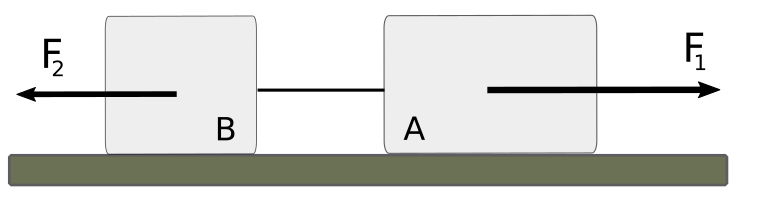
\includegraphics[scale=0.35]{../03_Dinamika_materijalne_tocke/Zadatak_D308.png}
  \end{center}
  %\caption{Fish}
\end{figure}


